\section{Geometrical Interpretation}
\label{geometry}

In this section we want to develop some geometrical intuition behind the
evaluation methods criteria and the imputation models, as well as why a
missing data problem requires different methods from an usual inference
problem.

Take a multivariate time series of daily log returns:
\[
R =
\begin{pmatrix}
r_1^\top \\
r_2^\top \\
\vdots \\
r_T^\top
\end{pmatrix}
=
\begin{pmatrix}
r_{11} & r_{12} & \cdots & r_{1N}\\
r_{21} & r_{22} & \cdots & r_{2N}\\
\vdots & \vdots & \ddots & \vdots\\
r_{T1} & r_{T2} & \cdots & r_{TN}
\end{pmatrix}
\in\mathbb{R}^{T\times N}
\]

The (t)-th observation is:

\[
r_t =
(r_{t1},\ldots,r_{tN})^\top
\in\mathbb{R}^N
\]

The (i)-th variable asset realization is:

\[
R_i =
(r_{1i},\ldots,x_{Ti})^\top
\in\mathbb{R}^T
\]

Let us first consider each asset separately.
We interpret each asset return series as a finite-sample realization of an underlying square-integrable random variable
in a Hilbert space:

\[
R_i \in
L^2(\Omega,\mathcal{F},\mathbb{P})
=
\left\{
X:\Omega\rightarrow\mathbb{R}
:
\mathbb{E}[X^2]<\infty
\right\}
\]

Square integrability, which is a reasonable assumption \footnote{Empirical work as \cite{plerou1999} shows
that the power law exponent of individual stocks is around 3, meaning variance exists but skew and kurtosis may not.},
enables us to define an useful inner product
on $L^2$, namely:
\[
\langle X,Y\rangle
\eqqcolon
\mathbb{E}[XY]
\]

This is remarkably similar to the definition of covariance, and is equal when the mean
of $X$ and $Y$ is zero; at the daily level this is almost the case. We can use this
approximation to see that the covariance and correlation of two assets are a function
of their angle in $L^2$:

\[
\langle X,Y\rangle
\simeq
\operatorname{Cov}(X,Y)
\]

\[
\rho(X,Y)
=
\frac{\operatorname{Cov}(X,Y)}{\operatorname{Var}(X)\operatorname{Var}(Y)}
\simeq
\frac{\langle X,Y\rangle}
{\|X\|\|Y\|}
=\cos(\theta)
\]

The crucial part of this thesis is making sure that this linear geometry is preserved
when imputing the missing data. The covariance matrix is of course the main
object of discussion, especially since it is used so widely across finance. It is
immediate that MSE is the squared distance of two assets.
The other metrics like VaR have no easy interpretation in this space.

\begin{figure}

  \centering
  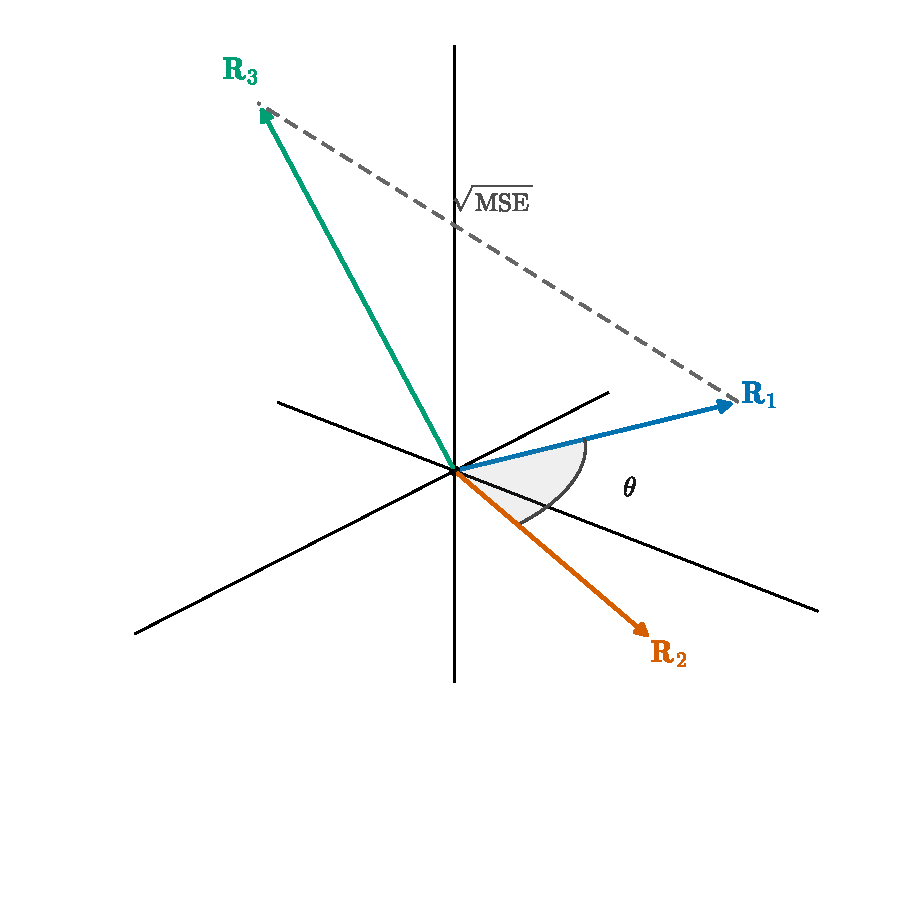
\includegraphics[width=0.5\textwidth]{Figures/hilbert_vectors.pdf}
  \caption{Returns as vectors in $L^2$}
  \label{fig:hilbert}
\end{figure}

Figure \ref{fig:hilbert} is an attempt to represent this abstract space. Now let us
turn to the realized space $\mathbb{R}^T$: the definitions above still apply, bar
the due discretizations, but now we can represent the missing data as a projection
of the full data.
Write:
\[
R_i=P_{\mathcal O_i}R_i+P_{\mathcal M_i}R_i = R_{O_i} + R_{M_i}
\]

Where $P_{\mathcal O_i}$ is the operator that deletes the missing data and $P_{\mathcal M_i}$
is the one that keeps it and deletes the observed one. Their ranges are clearly orthogonal under
the usual inner product.
The goal of our models is to approximate $R_{M_i}$ with:

\[
\hat{R}_{M_i} = h_\theta(R_{O_i}, R_{O_k \neq i})
\]

If we knew the values of $R_{M_i}$ we could run an approximation in the least
squares sense. Given $h_\theta$, find:
\[
\min_\theta\|{R}_{M_i}-\hat{R}_{M_i}\|
\]

This is essentially equivalent to trying to approximate the conditional expectation,
or in geometric terms projecting ${R}_{M_i}$ onto the space of functions $\sigma (R_{O_i}$ and $R_{O_k \neq i})$,
a subspace of $L^2$.

\begin{figure}

  \centering
  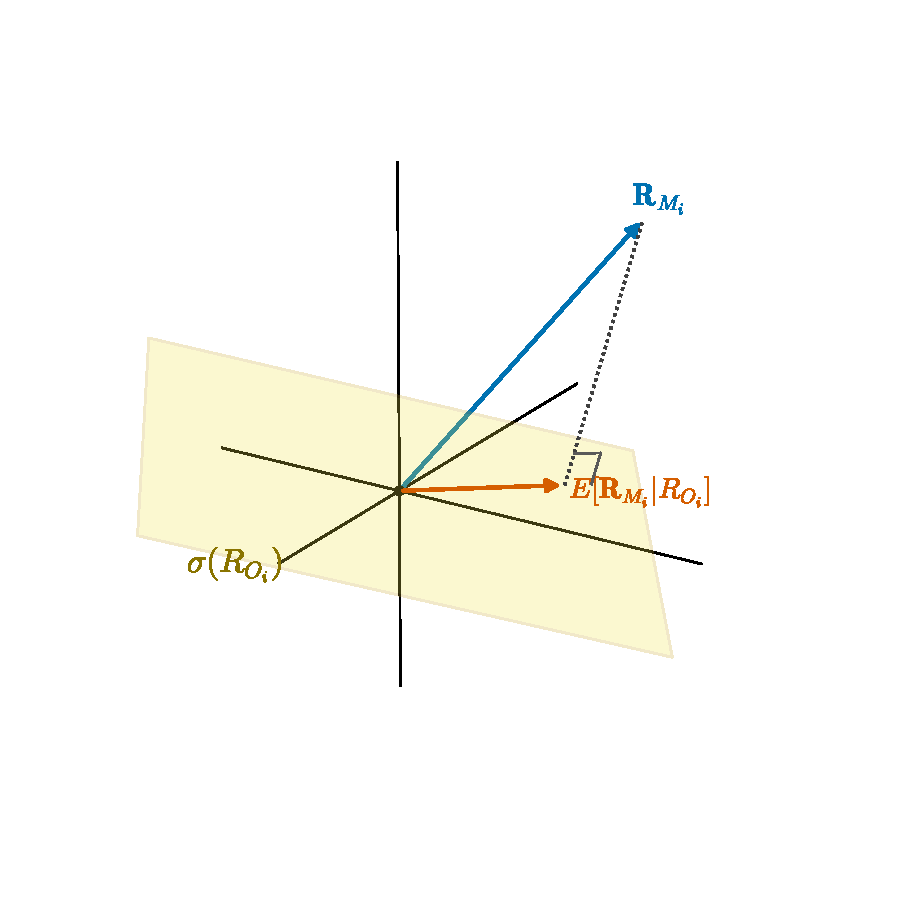
\includegraphics[width=0.7\textwidth]{Figures/projection_H.pdf}
  \caption{Conditional expectation as a projection}
  \label{fig:conditional}
\end{figure}


\clearpage

Let 
\[
R_i=(r_{1i},\ldots,r_{Ti})^\top\in\mathbb R^T
\]
denote the complete return vector of asset \(i\). Suppose that some entries of
\(R_i\) are missing. We denote by
\[
\mathcal O_i=\{t\in\{1,\ldots,T\}: r_{ti}\text{ is observed}\}
\]
the set of observed time indices, and by
\[
\mathcal M_i=\{t\in\{1,\ldots,T\}: r_{ti}\text{ is missing}\}
\]
the set of missing time indices.

For any subset \(A\subseteq\{1,\ldots,T\}\), define the coordinate projection
\(P_A:\mathbb R^T\to\mathbb R^T\) by
\[
(P_A x)_t=
\begin{cases}
x_t, & t\in A,\\
0, & t\notin A.
\end{cases}
\]
Then the complete return vector decomposes as
\[
\boxed{
R_i=P_{\mathcal O_i}R_i+P_{\mathcal M_i}R_i.
}
\]
The first term \(P_{\mathcal O_i}R_i\) is observed, while the second term
\(P_{\mathcal M_i}R_i\) is unobserved.

Under the empirical inner product
\[
\langle X,Y\rangle_T=\frac1T\sum_{t=1}^T X_tY_t,
\]
the two components are orthogonal, because they have disjoint supports:
\[
\left\langle P_{\mathcal O_i}R_i,\,
P_{\mathcal M_i}R_i\right\rangle_T=0.
\]
Hence,
\[
\|R_i\|_T^2
=
\|P_{\mathcal O_i}R_i\|_T^2
+
\|P_{\mathcal M_i}R_i\|_T^2.
\]


\clearpage
A multivariate time series is represented as


Hilbert space

The Hilbert space of square-integrable random variables is



Inner product



Norm

\[
\|X\|
=
\sqrt{\langle X,X\rangle}
=
\sqrt{\mathbb{E}[X^2]}.
\]

Distance

\[
d(X,Y)
=
\|X-Y\|.
\]
Centered random variables

If

\[
\mathbb{E}[X]=0,
\qquad
\mathbb{E}[Y]=0,
\]

then

\[
\langle X,Y\rangle
=
\operatorname{Cov}(X,Y).
\]

Correlation

\[
\rho(X,Y)
=
\frac{\langle X,Y\rangle}
{\|X\|\|Y\|}.
\]

Angle between random variables

\[
\theta
=
\arccos\left(
\frac{\langle X,Y\rangle}
{\|X\|\|Y\|}
\right).
\]
Conditional expectation

Conditional expectation

\[
\mathbb{E}[X\mid\mathcal{G}].
\]

Projection interpretation

\[
\mathbb{E}[X\mid\mathcal{G}]
=
P_{L^2(\mathcal{G})}(X),
\]

where $(P_{L^2(\mathcal{G})})$ denotes the orthogonal projection onto the closed subspace $(L^2(\mathcal{G}))$.

Orthogonality condition

\[
X-
\mathbb{E}[X\mid\mathcal{G}]
\perp
L^2(\mathcal{G}).
\]

Equivalently,

\[
\mathbb{E}
\left[
\left(
X-
\mathbb{E}[X\mid\mathcal{G}]
\right)
Y
\right]
=
0,
\qquad
\forall
Y\in L^2(\mathcal{G}).
\]
Covariance matrix

Mean vector

\[
\mu
=
\mathbb{E}[X].
\]

Covariance matrix

\[
\Sigma
=
\mathbb{E}
\left[
(X-\mu)(X-\mu)^\top
\right].
\]

Sample covariance

\[
S
=
\frac1{T-1}
\sum_{t=1}^T
(x_t-\bar x)
(x_t-\bar x)^\top.
\]

Correlation matrix

\[
R
=
D^{-1/2}
\Sigma
D^{-1/2},
\]

where

\[
D
=
\operatorname{diag}
(\Sigma).
\]
Gram matrix

The Gram matrix of variables

\[
G
=
X^\top X.
\]

The Gram matrix of observations

\[
K
=
XX^\top.
\]
PCA

Eigenvalue decomposition

\[
\Sigma
=
Q
\Lambda
Q^\top.
\]

Projection onto first (k) principal directions

\[
\widehat X
=
XQ_kQ_k^\top.
\]

Low-rank approximation

\[
X
\approx
UV^\top.
\]
Mahalanobis geometry

Mahalanobis distance

\[
d_M(x,\mu)
=
\sqrt{
(x-\mu)^\top
\Sigma^{-1}
(x-\mu)
}.
\]

Squared Mahalanobis distance

\[
\delta
=
(x-\mu)^\top
\Sigma^{-1}
(x-\mu).
\]

Ellipsoid

\[
\mathcal{E}
=
\{
x:
(x-\mu)^\top
\Sigma^{-1}
(x-\mu)
\le c
\}.
\]
Partitioned covariance matrix
\[
\Sigma
=
\begin{pmatrix}
\Sigma_{oo}
&
\Sigma_{om}
\\
\Sigma_{mo}
&
\Sigma_{mm}
\end{pmatrix}.
\]

Conditional mean

\[
\mu_{m|o}
=
\mu_m
+
\Sigma_{mo}
\Sigma_{oo}^{-1}
(x_o-\mu_o).
\]

Conditional covariance

\[
\Sigma_{m|o}
=
\Sigma_{mm}
-
\Sigma_{mo}
\Sigma_{oo}^{-1}
\Sigma_{om}.
\]
Projection matrices

Orthogonal projector

\[
P
=
P^\top
=
P^2.
\]

Least-squares projection

\[
P
=
X
(X^\top X)^{-1}
X^\top.
\]

Projected vector

\[
\widehat y
=
Py.
\]

Residual

\[
r
=
(I-P)y.
\]

Orthogonality

\[
P(I-P)=0.
\]
Matrix norms

Frobenius norm

\[
\|A\|_F
=
\sqrt{
\sum_{i,j}
a_{ij}^2
}.
\]

Spectral norm

\[
\|A\|_2
=
\sigma_{\max}(A).
\]

Nuclear norm

\[
\|A\|_*
=
\sum_i
\sigma_i(A).
\]
Matrix completion

Projection operator

\[
P_\Omega(X).
\]

Optimization problem

\[
\min_M
\;
\frac12
\|
P_\Omega(X-M)
\|_F^2
+
\lambda
\|M\|_*.
\]
Student-(t) distribution
\[
X
\sim
t_\nu(\mu,\Sigma).
\]

Student-(t) weight

\[
w_i
=
\frac{\nu+p}
{\nu+\delta_i}.
\]
EM algorithm

Expected complete-data log-likelihood

\[
Q(\theta|\theta^{(k)})
=
\mathbb{E}
\left[
\log
p(X_{\rm obs},X_{\rm mis}\mid\theta)
\mid
X_{\rm obs},
\theta^{(k)}
\right].
\]

M-step

\[
\theta^{(k+1)}
=
\arg\max_\theta
Q(\theta|\theta^{(k)}).
\]
Random paths

A multivariate path

\[
X:
[0,T]
\rightarrow
\mathbb{R}^N.
\]

Time-parametrized market trajectory

\[
t
\mapsto
X_t.
\]
Signatures

Signature

\[
S(X)
=
\left(
1,
\int dX,
\int dX\otimes dX,
\int dX\otimes dX\otimes dX,
\ldots
\right).
\]

Truncated signature

\[
S^{(m)}(X).
\]

Signature distance

\[
d_{\rm sig}
=
\left\|
S^{(m)}(X)
-
S^{(m)}(\widehat X)
\right\|.
\]
Useful notation

Expectation

\[
\mathbb{E}[X].
\]

Probability

\[
\mathbb{P}(A).
\]

Variance

\[
\operatorname{Var}(X).
\]

Covariance

\[
\operatorname{Cov}(X,Y).
\]

Trace

\[
\operatorname{tr}(A).
\]

Determinant

\[
\det(A).
\]

Rank

\[
\operatorname{rank}(A).
\]

Diagonal matrix

\[
\operatorname{diag}(a_1,\ldots,a_n).
\]

Identity matrix

\[
I_n.
\]

Positive-definite matrices

\[
\mathcal{S}_{++}^n.
\]

Symmetric matrices

\[
\mathcal{S}^n.
\]